\documentclass[10pt]{exam}
\usepackage[phy]{template-for-exam}
\usepackage{tikz}
\usepackage[top=0.2in, bottom=0.5in, left=0.5in, right=0.4in]{geometry}


\begin{document}
\pagestyle{empty}

\def\mytitle{Ch 10 Test: Rotation}

\newcommand{\topmatter} {


  \vfill
  
  \section*{Instructions}

  \begin{enumerate}
    \item Put your name on this page and \textbf{bubble in your 8-digit Student ID number} (400....).
    \item Tear off this front page and the back page (which is the equation sheet).
    \item Put your name on the top of the rest of the packet.
    \item The problems are on the first two pages, the next page contains the bonus problem, and the next few pages contain the multiple choice.
    \item You may write on anything, but I'm only grading this page and the first three pages of the rest of the packet.
  \end{enumerate}

}

\newcommand{\drawscantron}[2]{
  \begin{tikzpicture}
    \node[anchor=south west] at (0,0) {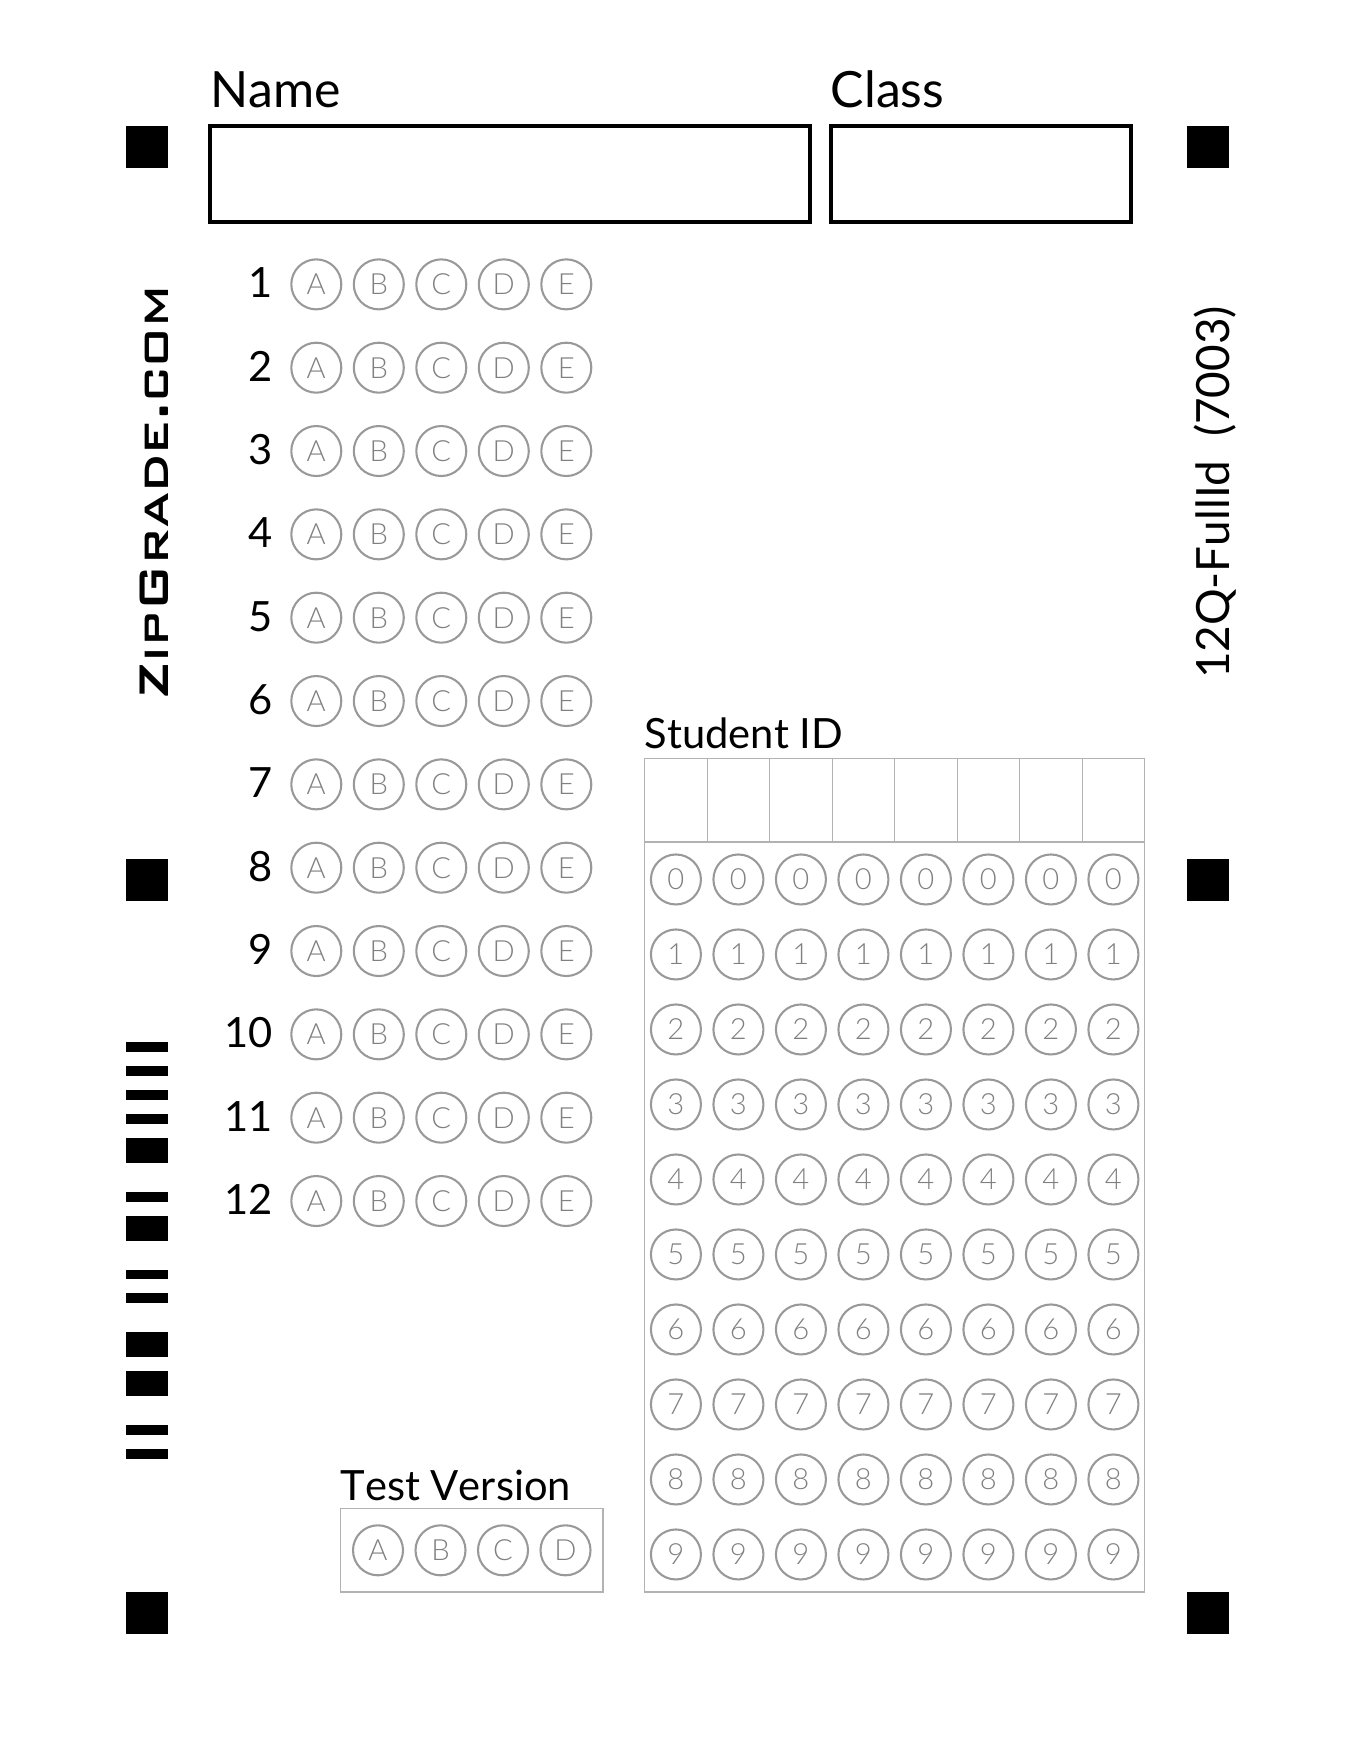
\includegraphics[height=5in]{12Q.png}};
    \fill (#1,#2) circle (0.2);
    \node[anchor=west] at (-8.6,12) {\LARGE \bf \sc \mytitle};
    \fill[white] (1.7,3.9) rectangle ++(2.8,1.1);
  \end{tikzpicture}
}



  \drawscantron{2.85}{1.65}
  \topmatter

\pagebreak

  \drawscantron{3.3}{1.65}
  \topmatter

\pagebreak

  \drawscantron{3.75}{1.65}
  \topmatter

\pagebreak

  \drawscantron{4.2}{1.65}
  \topmatter


\end{document}